% !TEX root = ../notes.tex

% ================ Introduction ==============
\section*{Course content}

The purpose of the course is to present multiple topics in the data science field such as \emph{Data Wrangling}, \emph{Data Management}, \emph{Data Mining}, \emph{Machine Learning}, \emph{Visualization}, \emph{Statistics} and \emph{Story telling}. The course has not the presumption to go deeply into each argument. It is due to the extent of the subject and the fact that it is evolving really quickly, hence learning in depth a specific tool will not pay off.

\subsection*{Skills to develop}

In this course, you will work, thus develop, the following skills:

\begin{description}
 \item \emph{Data mining/scraping/sampling/cleaning} in order to get an informative, manageable data setlength
 \item \emph{Data storage and management} in order to be able to access data quickly and reliably during subsequent analysis
 \item \emph{Exploratory data analysis} to generate hypotheses and intuition about the data
 \item \emph{Prediction} based on statistical tools such as regression, classification, and clustering
 \item \emph{Communication of results} through visualization, stories and interpretable summaries
\end{description}

\subsection*{Structure of the notes}

The notes of the lectures are put in writing with the aim of summarizing the main topics and concepts illustrated during the classes. To those who are curious, it points to external links that may help you to an in-depth understanding of the field. Each chapter corresponds to a lecture. The hope is that the work could be useful for the current and future students. 


\clearpage

\section{Introduction}

\subsection{What is Data Science?}

When we talk about Data Science, we often use the term Big Data as the enormous amount of data that exists in the world. But Big Data is not only about collecting huge amount of data. It is challenging but not enough. The real value comes from the insights. The {\it internet} companies (Google, Facebook, etc.) 
understood this many years ago.
\\ \\
An accurate definition of Data Analysis is given by Wikipedia:
\begin{framed}
{\it {\bf Analysis of data} is a process of {\bf inspecting}, {\bf cleaning}, {\bf transforming}, and {\bf modeling data} with the goal of {\bf discovering useful information}, suggesting conclusions, and supporting decision-making.
Data analysis has multiple facets and approaches, encompassing diverse techniques under a variety of names, {\bf in different business}, science, and social science {\bf domains}.}
\signed{\href{https://en.wikipedia.org/wiki/Data\_analysis}{Wikipedia - Data Analysis}}
\end{framed}

Therefore, a Data Scientist has to master different kinds of skills such as {\bf Mathematics} , {\bf Statistics}, {\bf Programming} and the {\bf Domain Expertise}. \href{http://videolectures.net/kdd2014\_conway\_social\_science/}{Drew Conway's Venn diagram}, Figure \ref{img:venn}, shows the different combination man can obtain with these three skills.

\begin{figure}[H]
 \centering
 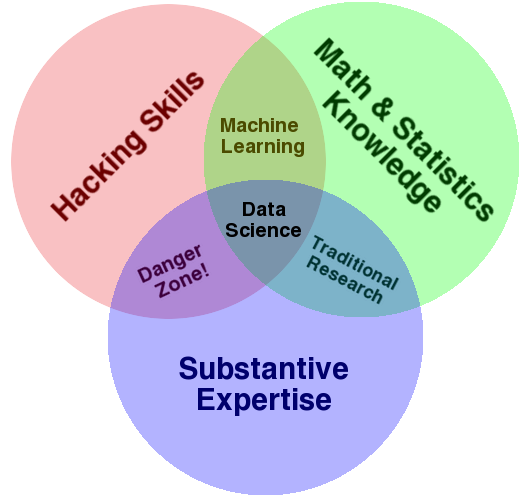
\includegraphics[width=7cm]{./pic/Data_Science_VD.png}
 \caption{\label{img:venn} Venn Diagram describing the different combination of skills used by a Data Scientist (by Drew Conway)} 
\end{figure}

\begin{figure}[H]
 \centering
 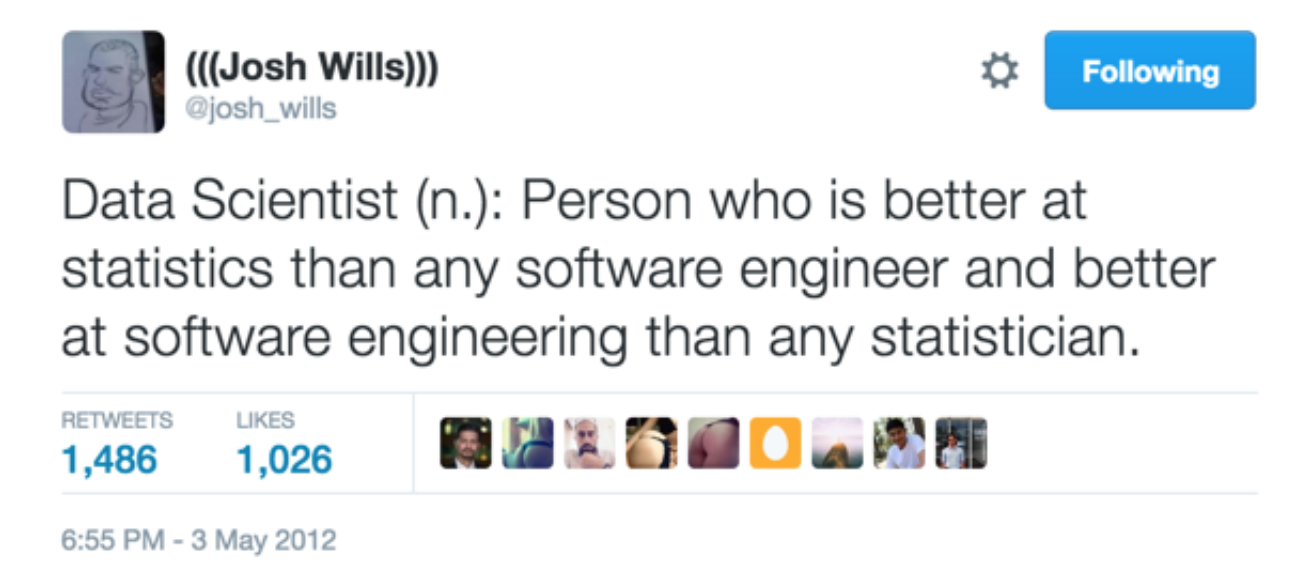
\includegraphics[width=10cm]{./pic/tweet_wills.png}
 \caption{\label{img:tweet_wills} A tweet from Josh Wills, Data Scientist at Slack.}
\end{figure}

{\bf A more practical definition} 

Data Science is about the whole processing pipeline to extract information out of data. As such, a Data Scientist {\bf understands and cares about the whole data pipeline}.

\begin{minipage}{0.5\textwidth}
\begin{figure}[H]
 \centering
 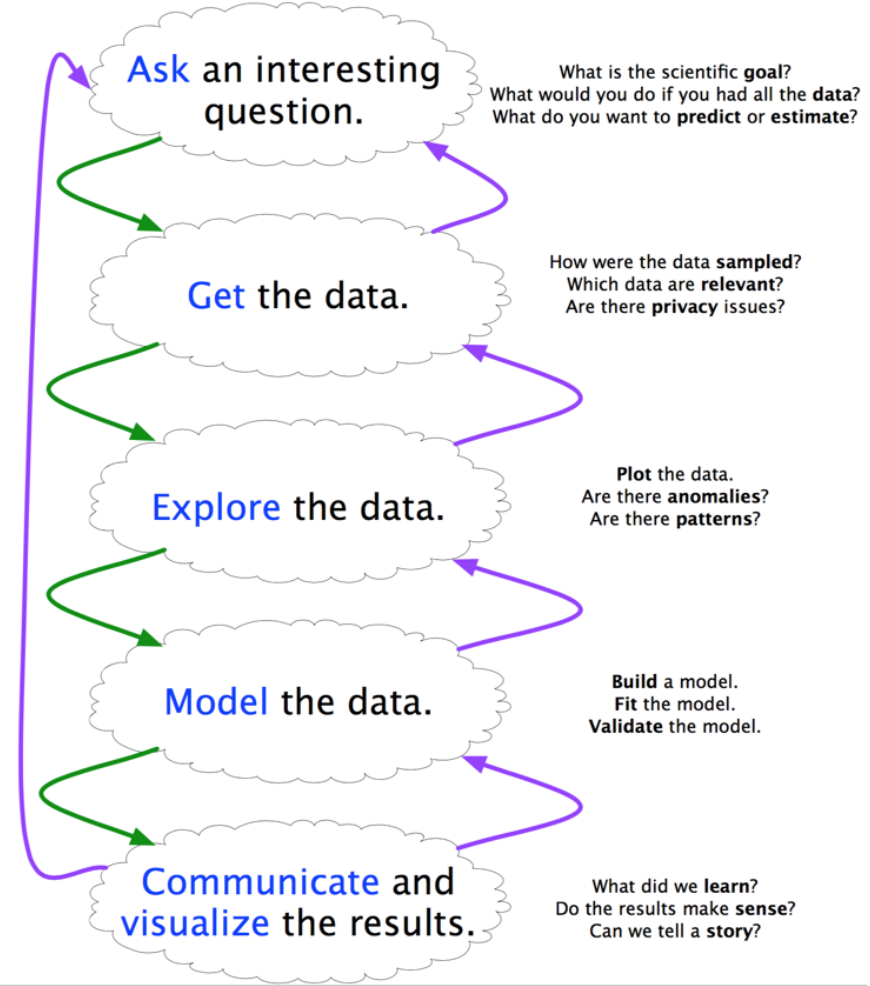
\includegraphics[width=8cm]{./pic/pipeline.png}
\end{figure}
\end{minipage} \hfill
\begin{minipage}{0.45\textwidth}
A {\bf data pipeline} consists of 3 steps:
\begin{enumerate}
 \item Preparing to run a model: \\
  {\it Gathering, cleaning, integrating, restructuring, transforming, loading, filtering, deleting, combining, merging, verifying, extracting, shaping}
 \item Running the model
 \item Communicating the results
\end{enumerate}
\vspace{0.5cm}
 A ``good'' Data Scientist will always go back and forth between the steps. The diagram on the left shows exactly what can happen. 
\end{minipage}
